\documentclass{article}

\usepackage{Sweave}
\begin{document}
\Sconcordance{concordance:ex9_AndreWerneck.tex:ex9_AndreWerneck.Rnw:%
1 2 1 1 0 9 1 1 14 1 1 1 8 1 2 4 1 1 145 1 1 1 4 1 2 1 1 1 2 4 0 1 2 7 %
1 1 2 1 0 1 5 2 0 1 3 1 0 3 1 1 2 3 1 1 2 1 1 1 140 139 0 1 2 2 1 1 2 4 %
0 1 3 5 1}


\title{Exercicio 9 - Redes Neurais Artificiais}
\author{Andre Costa Werneck}
\date{13/06/2022}
\maketitle
\newpage

Os dados foram gerados assim como especificado e, dessa forma, o modelo foi treinado com 45 amostras e testado com um conjunto de dados de 629 pontos. O ruido tambem foi acrescentado ao modelo, assim como requisitado. Os dados em forma de bolas azuis sao os dados de treinamento e a linha vermenlha representa o conjunto de testes. 

\begin{center}
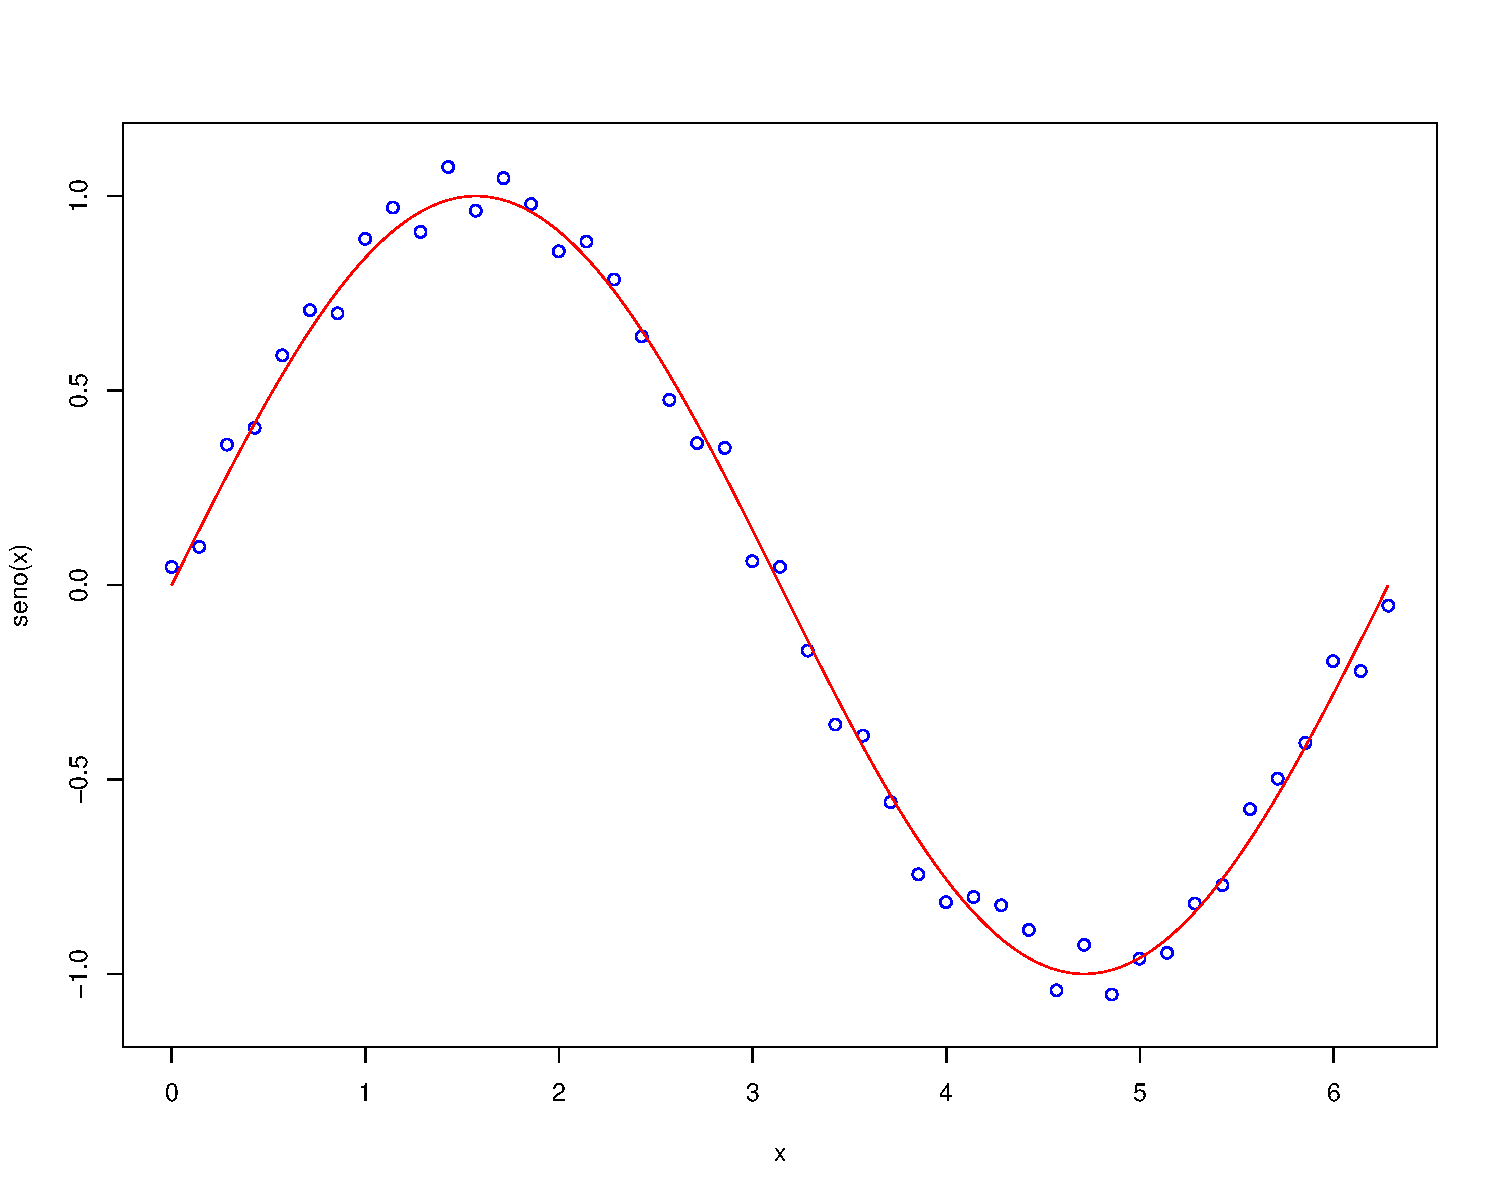
\includegraphics{ex9_AndreWerneck-002}
\end{center}

Apos isso, a rede MLP foi adaptada do que havia sido mostrado em sala de aula. Utilizou-se apenas uma camada de entrada (retirou-se a outra), acrescentou-se mais um neuronio na camada intermediaria (no total ficaram 3) e utilizou-se, logo, apenas uma saida na camada derradeira (retirou-se uma). Alem disso, utilizou-se uma funcao de custo linear na saida e a tanh na camada intermediaria. Dessa forma, a derivada da funcao de saida ficou igual a 1 e nao em sech2. 

Tendo isso em vista, executou-se a nova rede por 5 vezes e armazenou-se o valor do erro quadratico medio (MSE) de cada execucao. Logo, segue o resultado em imagem e, tambem, a media do MSE em conjunto com seu desvio padrao. 

\begin{center}
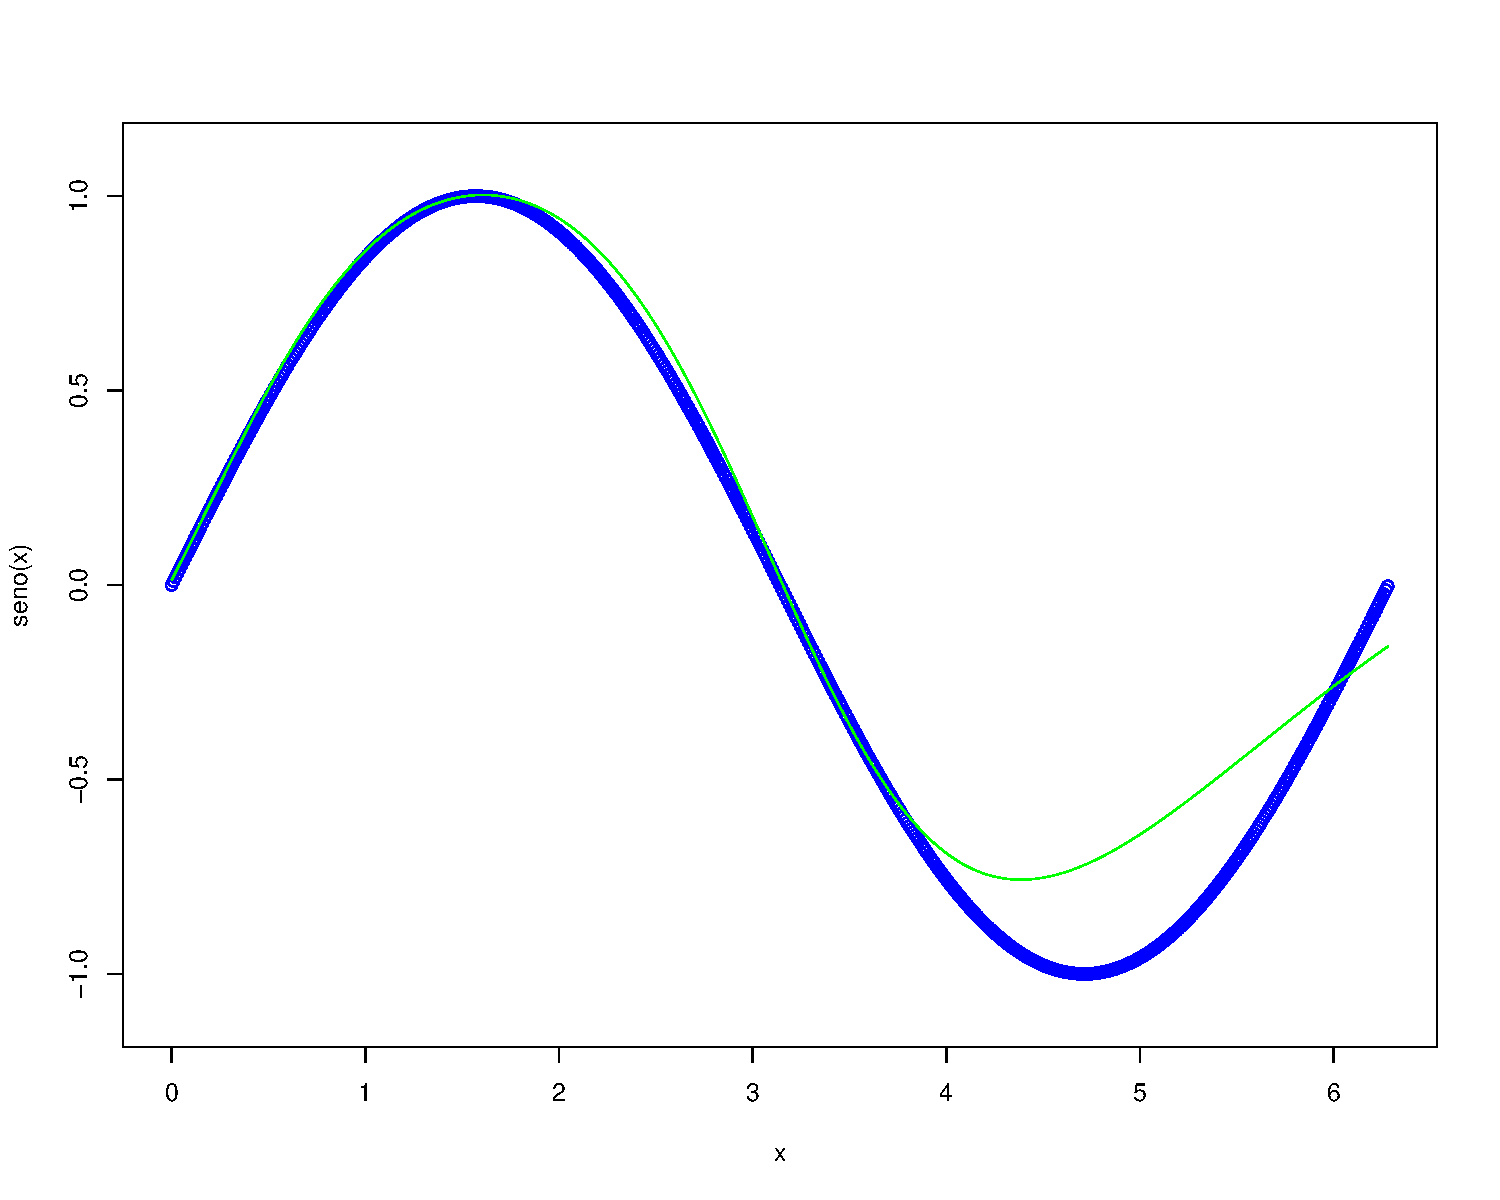
\includegraphics{ex9_AndreWerneck-004}
\end{center}

\begin{Schunk}
\begin{Soutput}
MSE = 0.0130184695947542 + - 0.00669742028344812
\end{Soutput}
\end{Schunk}

Dessa forma, conclui-se que, mesmo com uma certa divergencia da funcao geradora, o MSE medio ficou dentro de um valor baixo e, por isso, pode ser considerado que o presente experimento foi bem sucedido e foi, assim, verificada a aproximacao do seno a partir de uma rede MLP de 2 camadas e 3 neuronios na camada escondida.


\section{Anexos}

O codigo gerado durante a execucao do exercicio segue abaixo, assim como seus comentarios.

\begin{Schunk}
\begin{Sinput}
> rm(list = ls())
> sech2 <- function(u){
+   return(((2/(exp(u)+exp(-u)))*(2/(exp(u)+exp(-u)))))
+ }
> # generating data
> x <- as.matrix(seq(0,(2*pi),length = 45))
> ruido <- as.matrix(runif(dim(x)[1],min = -0.1,max = 0.1))
> y <- as.matrix(sin(x)) + ruido
> plot(x,y,xlim=c(0,(2*pi)),ylim = c(-1.1,1.1),xlab ='x',ylab = 'seno(x)',col='blue')
> xtest <- as.matrix(seq(0,(2*pi),by = (0.01)))
> ytest <- as.matrix(sin(xtest))
> par(new=T)
> plot(xtest,ytest,'l',xlim=c(0,(2*pi)),ylim = c(-1.1,1.1),xlab ='x',ylab = 'seno(x)',col='red')
> exec <- 5
> MSEvec <- matrix(nrow = 1,ncol = exec)
> for (k in 1:exec) {
+     
+   
+   # implementando o bakcpropagation
+   #bias
+   i1 <- 1
+   i3 <- 1
+   i4 <- 1
+   i5 <- 1
+   
+   # incializando aleatoriamente os pesos
+   w61 <- runif(1)-0.5
+   w62 <- runif(1)-0.5
+   
+   w72 <- runif(1)-0.5
+   w73 <- runif(1)-0.5
+   
+   w82 <- runif(1)-0.5
+   w84 <- runif(1)-0.5
+   
+   w95 <- runif(1)-0.5
+   w96 <- runif(1)-0.5
+   w97 <- runif(1)-0.5
+   w98 <- runif(1)-0.5
+   
+   # definindo os hps 
+   tol <- 0.01
+   nepocas <- 0
+   eepoca <- tol+1
+   eta <- 0.01
+   maxepocas <- 2500
+   N <- length(x) # numero total de linhas de x 
+   
+   evec <- matrix(nrow = 1,ncol = maxepocas)
+   
+   while((nepocas < maxepocas) && (eepoca > tol)){
+     
+     ei2 <- 0 
+     iseq <- sample(N)
+   
+     for(i in (1:N)){
+       
+       i2 <- x[iseq[i],1]
+       
+       y9 <- y[iseq[i],1]
+       
+       # neuronios camada intermediaria
+       u6 <- i1*w61 + i2*w62
+       u7 <- i3*w73 + i2*w72
+       u8 <- i4*w84 + i2*w82
+       
+       i6 <- tanh(u6)
+       i7 <- tanh(u7)
+       i8 <- tanh(u8)
+       
+       #neuronio de saida
+       u9 <- i5*w95 + i6*w96 + i7*w97 + i8*w98
+       
+       i9 <- u9
+       
+       #erro camada de saida
+       e9 <- y9 - i9
+       d9 <- e9*1
+       
+       # calculando o diferencial dos pesos
+       DW95 <- eta * d9 * i5
+       DW96 <- eta * d9 * i6
+       DW97 <- eta * d9 * i7
+       DW98 <- eta * d9 * i8
+       
+       # backpropagating
+       d6 <- (d9*w96)*sech2(u6)
+       d7 <- (d9*w97)*sech2(u7)
+       d8 <- (d9*w98)*sech2(u8)
+       
+       # calculando o diferencial dos pesos
+       DW61 <- eta*d6*i1 
+       DW62 <- eta*d6*i2
+       
+       DW72 <- eta*d7*i2
+       DW73 <- eta*d7*i3
+       
+       DW82 <- eta*d8*i2
+       DW84 <- eta*d8*i4
+       
+       # atualizando os pesos 
+       w61 <- w61 + DW61
+       w62 <- w62 + DW62
+       
+       w72 <- w72 + DW72
+       w73 <- w73 + DW73
+       
+       w82 <- w82 + DW82
+       w84 <- w84 + DW84
+       
+       w95 <- w95 + DW95
+       w96 <- w96 + DW96
+       w97 <- w97 + DW97
+       w98 <- w98 + DW98
+       
+       ei <- ((e9*e9))/1
+       ei2 <- ei2 + ei
+     }
+     
+     nepocas <- nepocas +1
+     evec[nepocas] <- ei2/N
+     eepoca<-evec[nepocas]
+     
+   }
+   
+   #plot(evec[1,(1:nepocas)])
+   
+   N <- dim(xtest)[1]
+   
+   yhatALL <- matrix(ncol = 1,nrow = N)
+   for(i in (1:N)){
+     i2 <- xtest[i,1]
+     # Saida  
+     y9 <- ytest[i, 1]
+     
+     # Camada intermediaria
+     u6 <- i1*w61 + i2*w62
+     u7 <- i2*w72 + i3*w73
+     u8 <- i2*w82 + i4*w84
+     
+     i6 <- tanh(u6)
+     i7 <- tanh(u7)
+     i8 <- tanh(u8)
+     
+     # Camada de saida
+     u9 <- i5*w95 + i6*w96 + i7*w97 + i8*w98
+     
+     i9 <- u9
+     
+     yhatALL[i,1] <- i9
+   }
+ 
+   MSEvec[1,k] <- (t(ytest-yhatALL) %*% (ytest-yhatALL))/dim(ytest)[1]
+   
+ }
> plot(xtest,ytest,xlim=c(0,(2*pi)),ylim = c(-1.1,1.1),xlab ='x',ylab = 'seno(x)',col='blue')
> par(new=T)
> plot(xtest,yhatALL,'l',xlim=c(0,(2*pi)),ylim = c(-1.1,1.1),xlab ='x',ylab = 'seno(x)',col='green')
> glue::glue("MSE = {mean(MSEvec)} + - {sd(MSEvec)}\n")
> 
\end{Sinput}
\end{Schunk}





\end{document}
